\section{Ships, Spacelanes, and Path Finding}
\label{sec:pathfinding}

The specification made it clear --- by the way weapons and navigation between planets was to be structured --- that ship motion needed to be relatively detailed. It is no use having a weapon that can be only used in one arc if ships could instantly pivot on the spot. Instead it was desired for ships to move as large objects with a great deal of momentum, with large turning circles and ponderous movements. However it would be undesirable for the motion of ships to be too realistic, as it would make the game needlessly difficult and confusing. A real object undergoing acceleration in space could of course, accelerate essentially indefinitely (until it was nearing the speed of light) but would need to take an equal amount of time to decelerate to stop again.

\begin{marginfigure}
	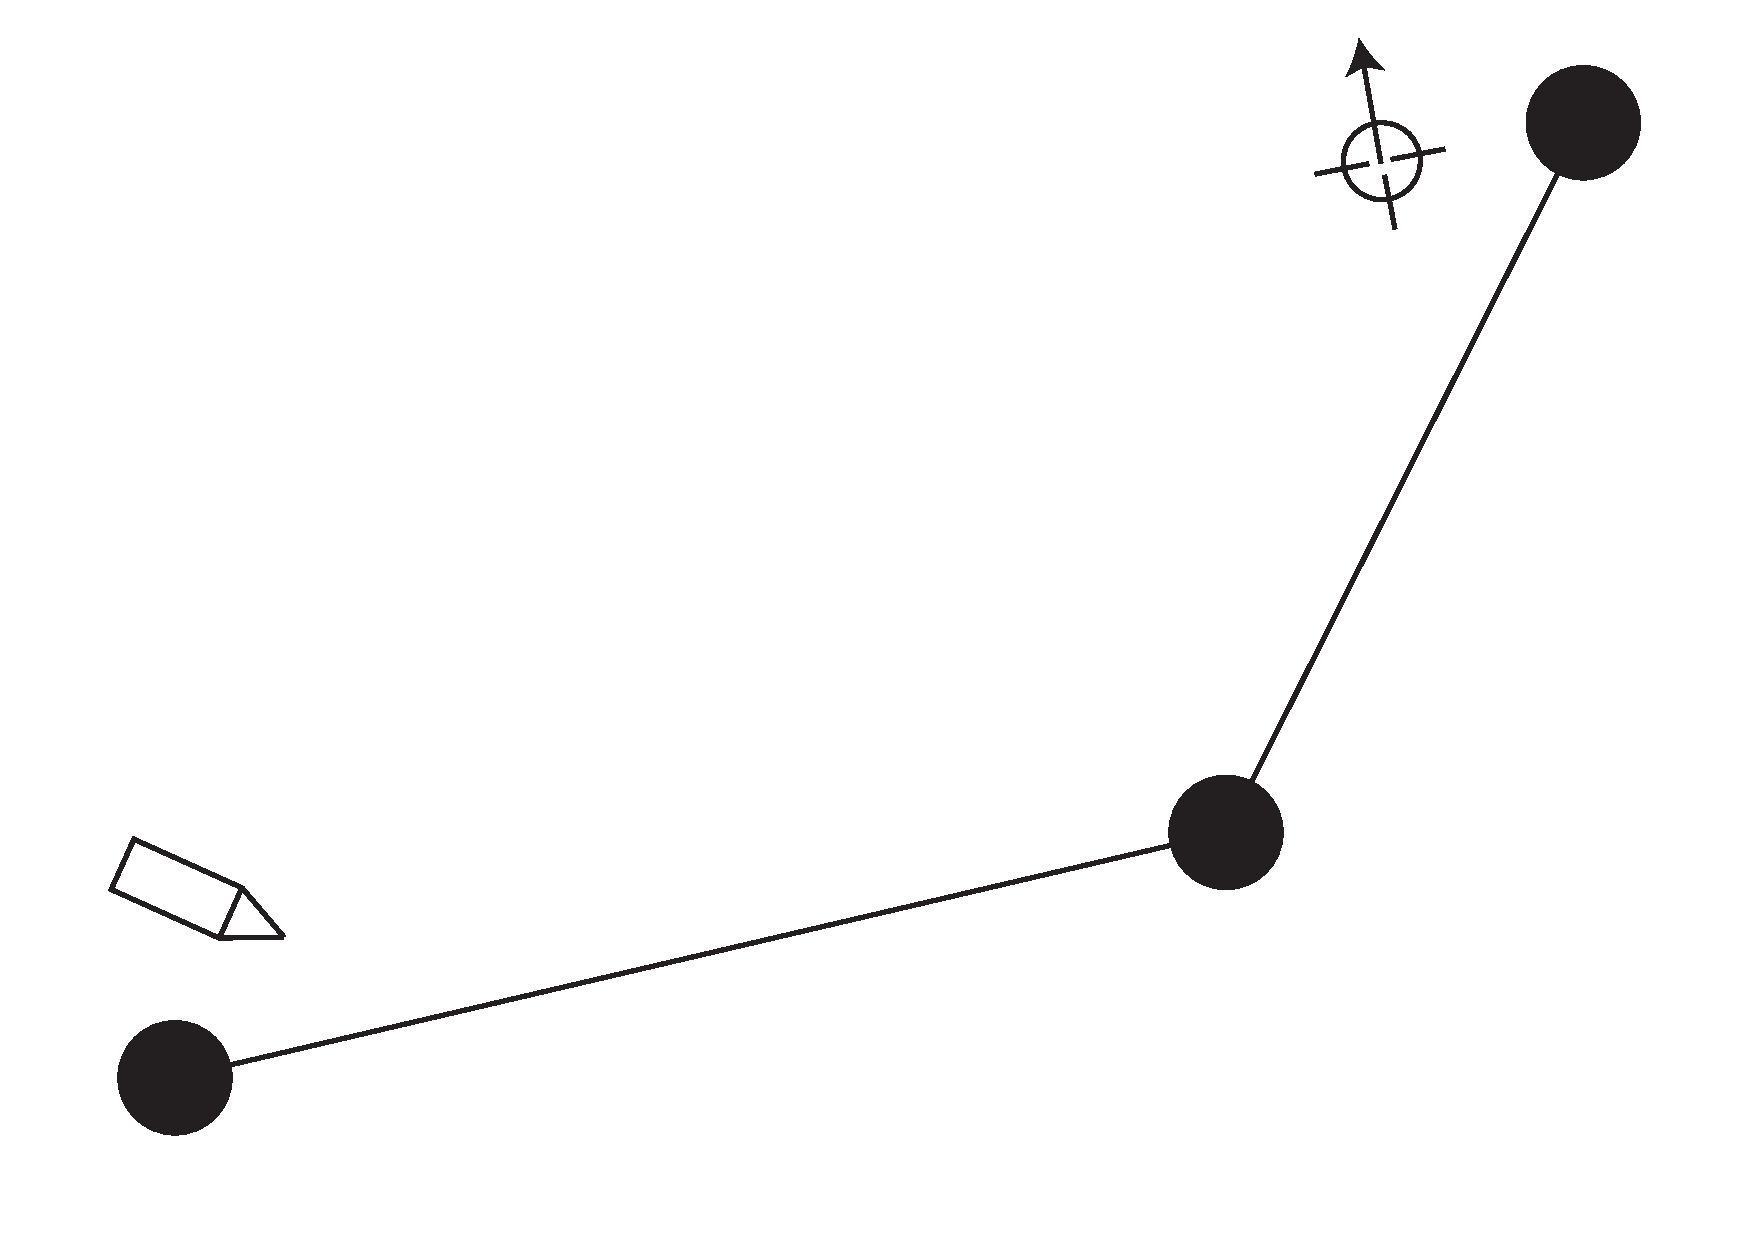
\includegraphics[width=20em]{res/pathfinding/spacelanes}
	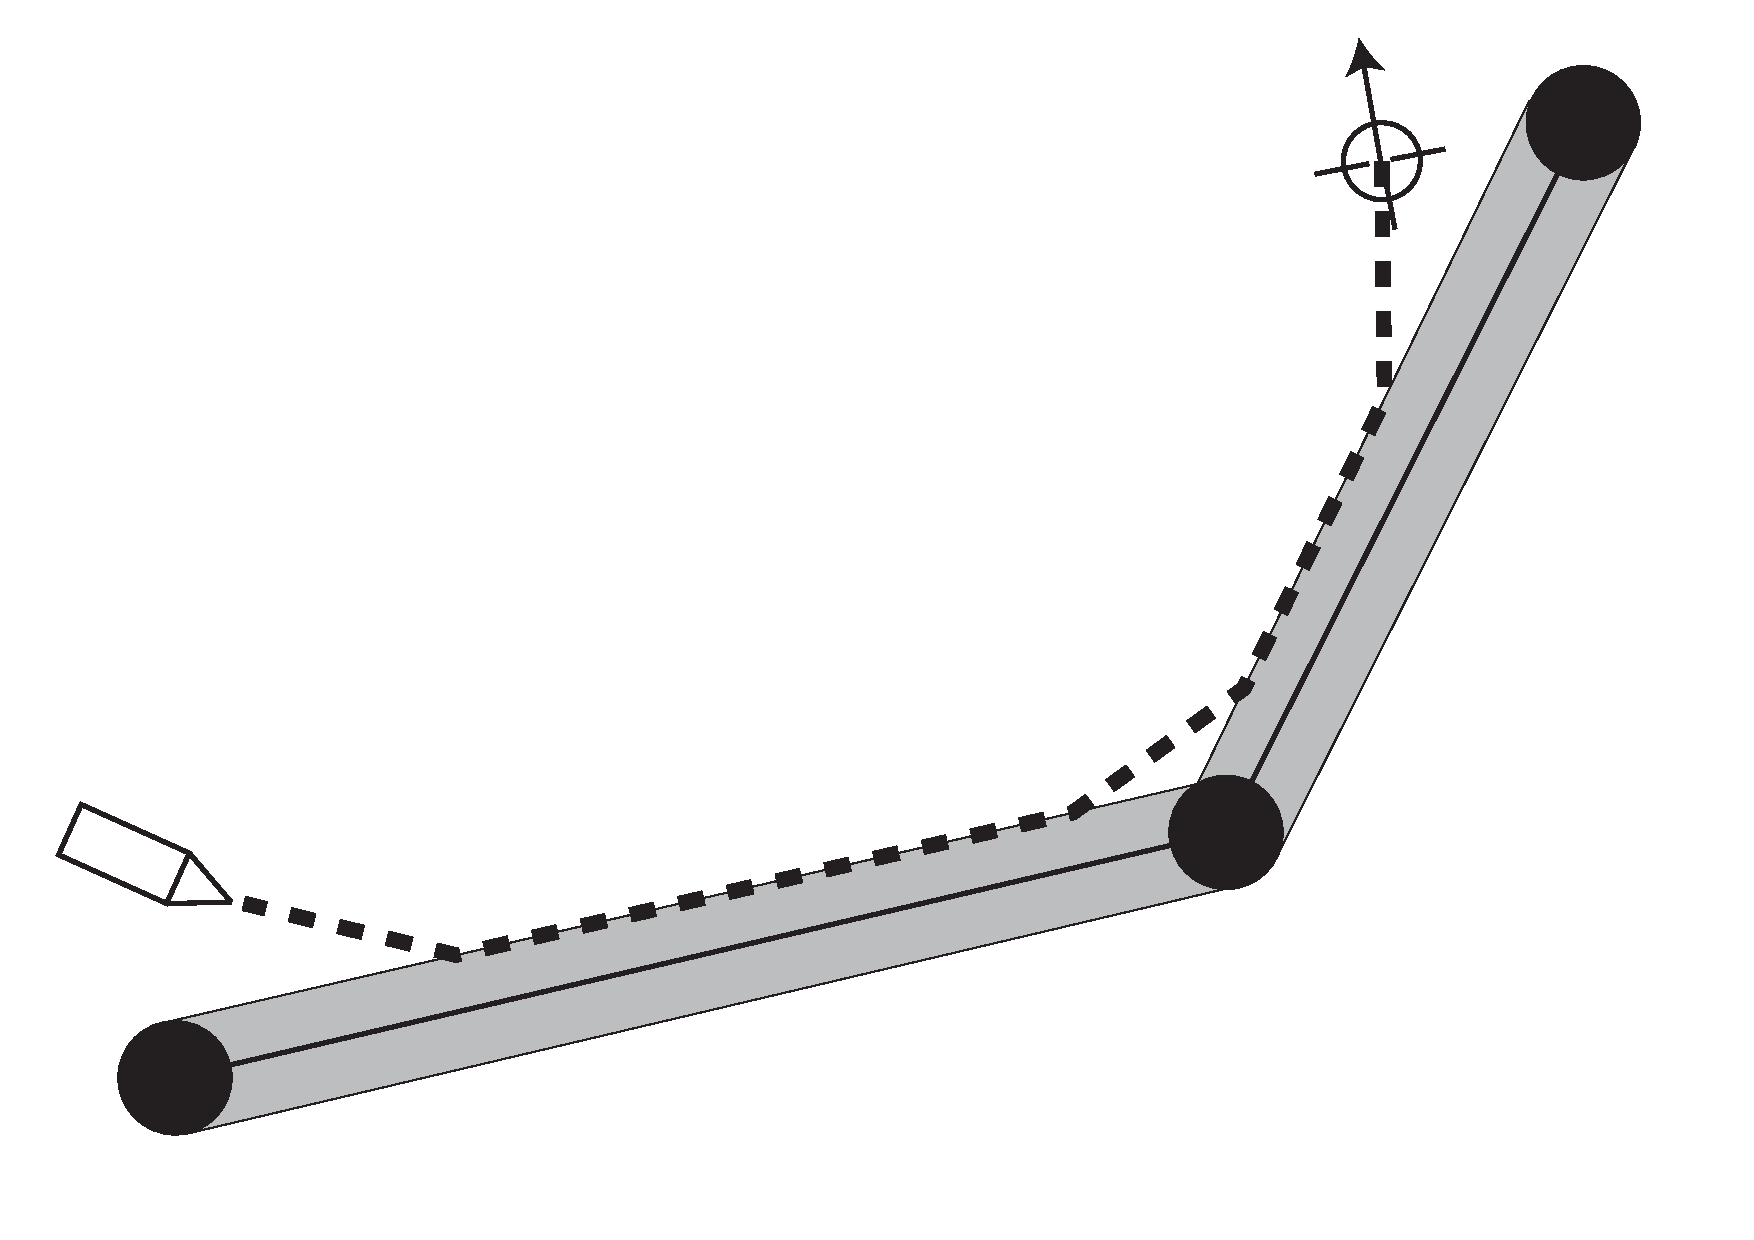
\includegraphics[width=20em]{res/pathfinding/spacelanes_ray}
	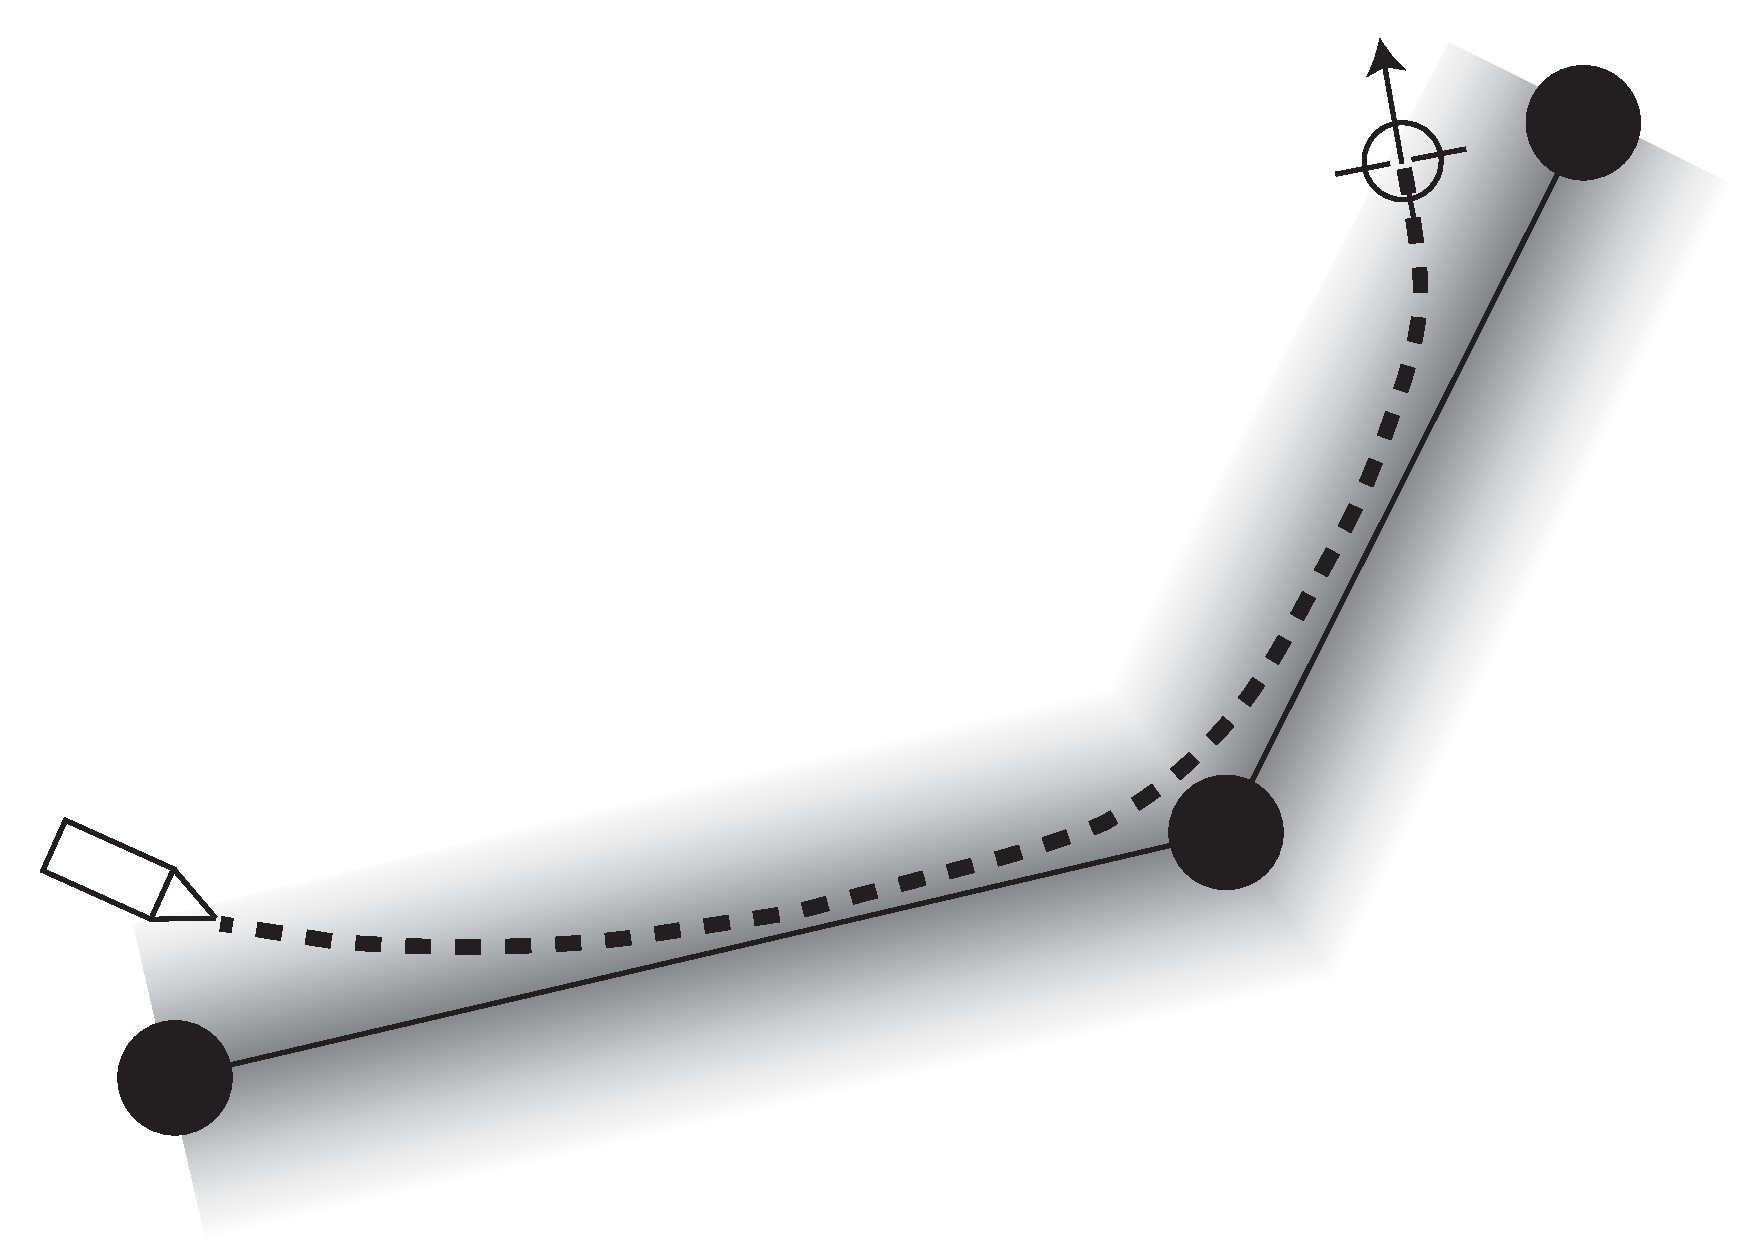
\includegraphics[width=20em]{res/pathfinding/spacelanes_field}
	\caption[Illustrations of different models for a path between current location and target utilising a spacelane]{Illustrations of different models for a path between current location and target utilising a spacelane.}
	\label{fig:spacelanes}
\end{marginfigure}

Intimately related to these questions is the precise nature of the \emph{spacelane} mechanics. Spacelanes between planets were introduced into the game in order for the otherwise empty space between planets to have some strategic topology, the idea being that the spacelanes can be traversed much more quickly than empty space. and so control of the lanes are vital to a successful strategy. Many different models were discussed for this mechanic during design meetings, both from the point of view of the in universe explanation, and the precise way in which the game would implement it. Initial ideas on the physical mechanism of the spacelane was that they conferred an additional optional acceleration: i.e. that if a ship is approximate to a lane it could opt to undergo greater acceleration than a ship far from a lane. But as mentioned, accurately modelling acceleration in space is somewhat contrary to the gameplay aspirations of the design. 

A simpler mechanic for ships that was considered to be more suitable, is for them to have a top speed that they could reach relatively quickly; but for them to still have large turning circles. This makes their motion more similar to naval ships engaged in warfare. The interpretation of the spacelane in this model cannot be simply a gain in acceleration as this confers little benefit. Instead it is clear that the spacelane must confer an addition to top speed. A possible physical interpretation of these behaviours is that the ships are moving in some kind of ether with friction, and so will reach a terminal velocity. The spacelane is then an area with an artificially induced lower density of ether.

Another fundamental question about the nature of the spacelane is whether its effects are immediately felt at full strength at a certain distance from it, or whether they fall off related to distance. the former is most definitely simpler, but the latter feels more natural as a mechanism. Figure~\ref{fig:spacelanes} shows the difference in the shortest paths that these approaches may generate, discounting the additional issue of ship turning.

\subsection{Algorithms for Pathfinding}
% physics hard
% bezier (not trivial)
% flow fields

Physical simulation of a large mass moving and turning in space was the initially preferred implementation method, but it became increasingly clear that this was going to be difficult both from an implementation and a user perspective. And while modelling the spacelane as having a continuous, field like nature, it was not at all clear how this would be achieved. It was decided to instead merely approximate the desired behaviour using bezier curves.

\begin{marginfigure}
	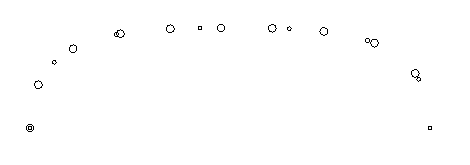
\includegraphics[width=20em]{res/pathfinding/bezier}
	\caption[Bezier path at regular intervals]{Bezier path at regular intervals (small circles) and the same path after having been reparameterisated by arc length (large circles).}
	\label{fig:bezier}
\end{marginfigure}

Over the Christmas break the code for a ship moving between two arbitrary points and headings was developed. Coding bezier paths themselves was not difficult, but moving an object continuously along one at a constant speed was much more complicated than expected. The accurate solution of this problem is called reparameterisation by arc length, and requires a solving a differential equation, but the method eventually used in Serenity was a numerical interpolation. Results are shown in Figure~\ref{fig:bezier}.

\begin{marginfigure}
	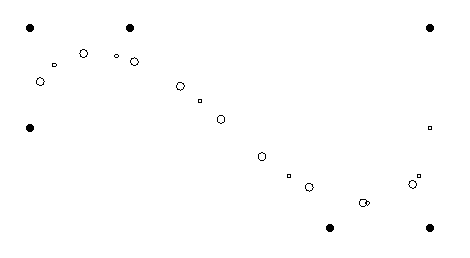
\includegraphics[width=20em]{res/pathfinding/bezierpath}
	\caption[Bezier path at regular intervals]{Bezier path at regular intervals (small circles) and the same path after having been reparameterisated by arc length (large circles).}
	\label{fig:bezierpath}
\end{marginfigure}

Even with the ability to move a ship smoothly along a given path, the selection of the path still required some considerable thought. An example of the control points generated for a move is shown in Figure~\ref{fig:bezierpath}.

\subsection{Applying A* to a Sector}
% what is the problem
% why this is no trivial problem
% Why A*

Applying a pathfinding algorithm to a sector has two stages: generating a graph which represents the sector, and running the algorithm that traverses the graph to find the shortest route to the destination. The algorithm chosen for the second stage is A* because it will always find the optimal solution (assuming the heuristic is admissible) and, if an efficient heuristic is used, then it is very fast too. However, the difficulty of using A* is that it requires a discrete graph to navigate, but the sector is not discrete as ships can move anywhere within it. The planets and spacelanes provide some points of reference, but they do not restrict the movement of the ships. Therefore, it is necessary to build a discrete graph from the sector model during stage one.

Just using the planets as nodes connected by edges of spacelanes does not work since the ships can go into other areas of space not covered by such a graph. Advanced techniques such as constructing a navigation mesh or a waypoint graph do not really apply in this situation since there are no obstacles for graphs to be built from. So, the solution was to take the simplistic graph generated only from the planets and spacelanes, and then add extra nodes and edges where appropriate. Extending the graph with these extra nodes was the difficult problem that had to be solved.

\begin{figure*}[h!]
	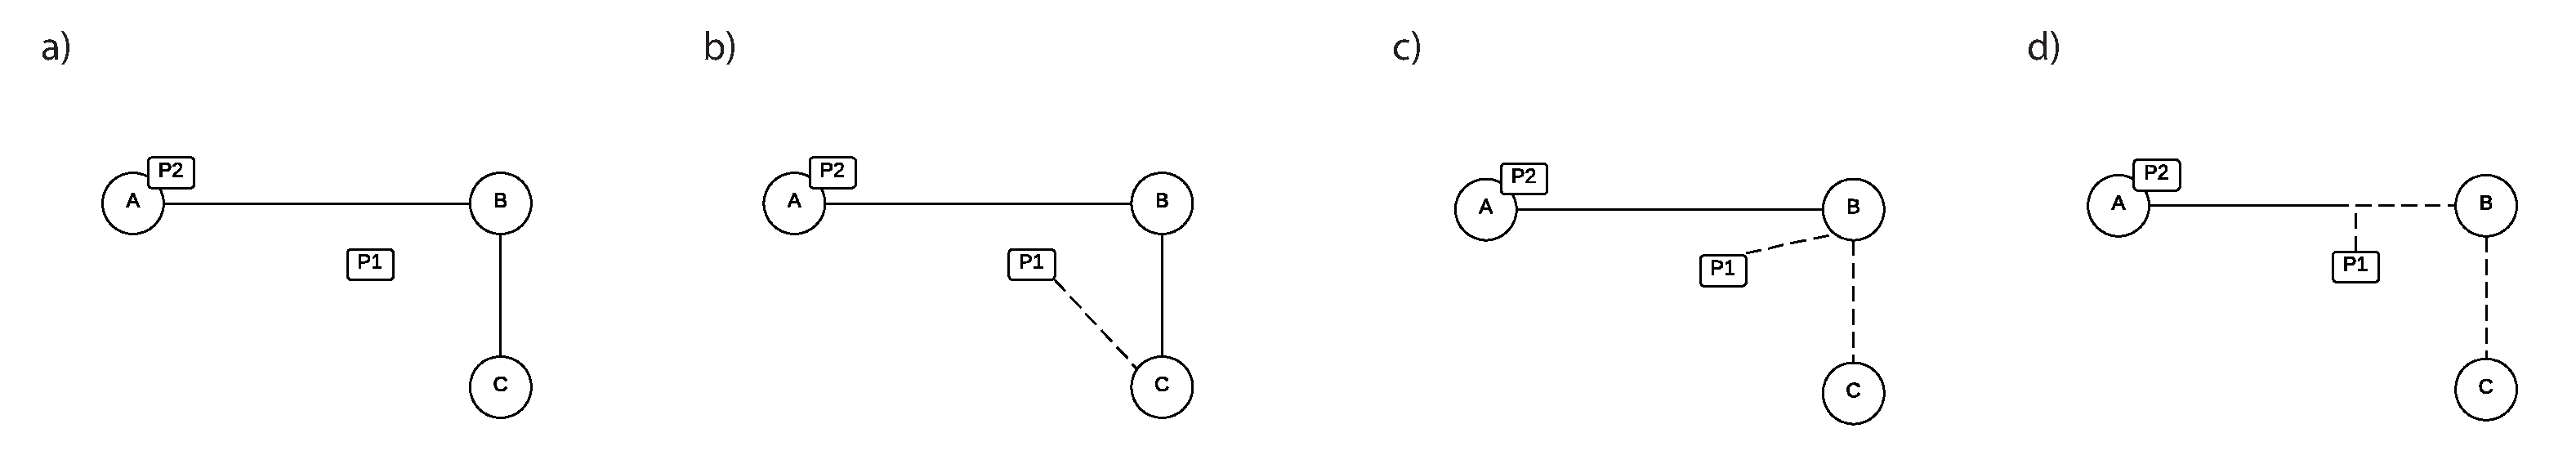
\includegraphics{res/pathfinding/PathFindingExample.pdf}
	\caption[Potential ship routes]{Potential routes a ship could take to reach its destination.}
	\label{fig:pathfindingexample}
\end{figure*}

First a typical ingame situation was taken to be analysed for the possible routes that a ship could take. Figure~\ref{fig:pathfindingexample} shows such a scenario. Figure~\ref{fig:pathfindingexample} (a) shows the location of two ships, $P_1$ and $P_2$, and three planets, $A$, $B$, and $C$, connected by spacelanes. If both ships want to reach planet $C$ then it is obvious which route $P_2$ will take, it can travel along spacelanes from $A$ to $B$ to $C$. However, there are three different possibilities for ship $P_1$:

\begin{enumerate}
	\item Go directly to planet $C$, shown in (b).
	\item Go to the closet planet, $B$, and then follow the spacelane to $C$, shown in (c).
	\item Travel to the nearest spacelane, between $A$ and $B$, and then follow the spacelanes to $C$, shown in (d).
\end{enumerate}

Travelling across open space is always going to be considerably slower than using spacelanes, so option one can be immediately be discarded as suboptimal. However, how fast are spacelanes? Is it best to greedily use spacelanes as much as possible or is it sometimes faster to travel a little longer through open space to reach a spacelane closer to the destination. Spacelanes have a multiplier effect on the speed of a ship so that a ship travelling along a spacelane speeds up $x$ times compared to its usual speed, where $x$ is a parameter defined by the sector model.

Suppose that $x$ is very large or infinite then travel along spacelanes with be almost instantaneous. Under these circumstances option three will be the optimal route since the least time is spent travelling off of spacelanes. However, for a lower value of $x$, option two will be optimal since the reduced distance to reach planet $B$ outweighs the benefits of the spacelane. Therefore, it is obvious that the heuristic cost function used by A* must take the multiplier effect of the spacelanes into account:

\begin{equation*}
	cost = \frac{distance}{speed \times multiplier}
\end{equation*}

Where the $distance$ between two nodes is simply the Euclidean distance. Using this cost function it becomes easier to find a good route by adding `virtual nodes' to the graph on nearby spacelanes and then using the A* algorithm to compare the costs of this extended graph. For example, in the scenario shown in Figure~\ref{fig:pathfindingexample} a virtual node is added to the spacelane between $A$ and $B$. This suggests a simple set of rules for adding new nodes:

\begin{enumerate}
	\item If the start point is in open space then add a node at the closest point on the closest spacelane
	\item If the destination is in open space then add a node at the closest point on the closest spacelane
\end{enumerate}

\begin{marginfigure}
	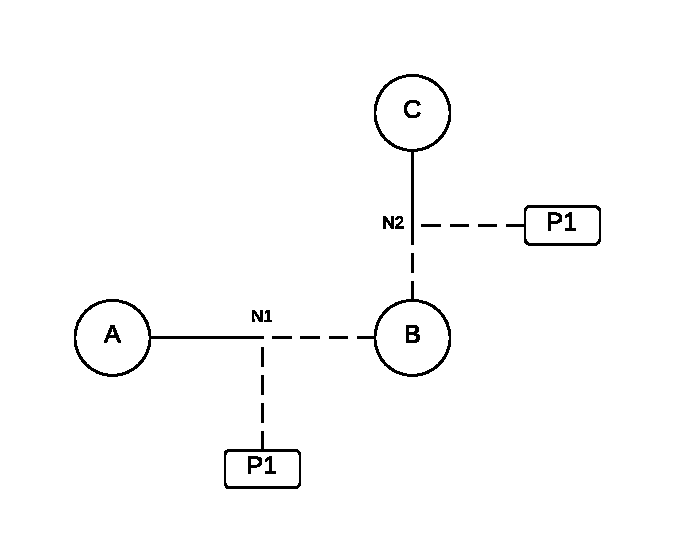
\includegraphics{res/pathfinding/PathFindingSector3.pdf}
	\caption[Adding nodes to the nearest spacelanes]{Adding nodes to the nearest spacelanes.}
	\label{fig:addingnodes}
\end{marginfigure}

For example, Figure~\ref{fig:addingnodes} shows how two nodes are added at $N_1$ and $N_2$ if a ship wants to go from $P_1$ to $P_2$. The graph is then completed to make all of the sensible routes connected. Using the same example from Figure~\ref{fig:addingnodes} it means that edges will be added between the $P_1$ and $N_1$, $P_2$ and $N_2$, $P_1$ to $B$, $B$ to $P_2$, and so on. The A* algorithm, using the simple cost function, can then be applied to this fully connected graph to find the best possible route to the destination.

\begin{marginfigure}
	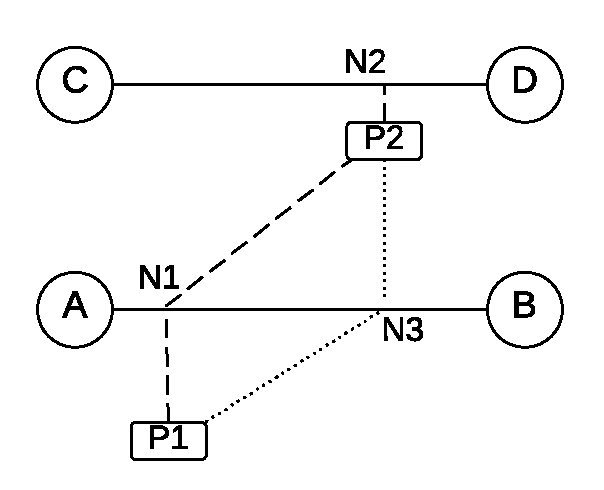
\includegraphics{res/pathfinding/NearestSpaceLaneUseless.pdf}
	\caption[The closest point on the closest spacelane is not always your friend]{The closest point on the closest spacelane is not always your friend.}
	\label{fig:uselessspacelane}
\end{marginfigure}

However, these two rules are too simplistic and will not provide the best route in all cases. Figure~\ref{fig:uselessspacelane} shows an example in which a ship wants to travel from $P_1$ to $P_2$. The current ruleset will add nodes $N_1$ and $N_2$ since they are the closest points on the nearest spacelanes. However, it is actually quicker to travel via $N_3$ than it would be to go straight from $N_1$ to $P_2$. There are just too many possibilities for quicker routes as the edge cases keep on building up. Therefore, it was decided to use a brute force solution that involves adding nodes at regular intervals along the nearest spacelanes. The best added node may not match the optimal solution exactly, but it will be better than the majority of other options. Using brute force is also not a highly desirable technique, but it works fast enough for this use case for now as further designing would have been required to reach a better solution.

Now that a discrete graph has been generated to represent the sector it can be fed to the A* algorithm which will find an optimal solution for the graph it has been presented.
